% Options for packages loaded elsewhere
\PassOptionsToPackage{unicode}{hyperref}
\PassOptionsToPackage{hyphens}{url}
%
\documentclass[
]{book}
\usepackage{lmodern}
\usepackage{amssymb,amsmath}
\usepackage{ifxetex,ifluatex}
\ifnum 0\ifxetex 1\fi\ifluatex 1\fi=0 % if pdftex
  \usepackage[T1]{fontenc}
  \usepackage[utf8]{inputenc}
  \usepackage{textcomp} % provide euro and other symbols
\else % if luatex or xetex
  \usepackage{unicode-math}
  \defaultfontfeatures{Scale=MatchLowercase}
  \defaultfontfeatures[\rmfamily]{Ligatures=TeX,Scale=1}
\fi
% Use upquote if available, for straight quotes in verbatim environments
\IfFileExists{upquote.sty}{\usepackage{upquote}}{}
\IfFileExists{microtype.sty}{% use microtype if available
  \usepackage[]{microtype}
  \UseMicrotypeSet[protrusion]{basicmath} % disable protrusion for tt fonts
}{}
\makeatletter
\@ifundefined{KOMAClassName}{% if non-KOMA class
  \IfFileExists{parskip.sty}{%
    \usepackage{parskip}
  }{% else
    \setlength{\parindent}{0pt}
    \setlength{\parskip}{6pt plus 2pt minus 1pt}}
}{% if KOMA class
  \KOMAoptions{parskip=half}}
\makeatother
\usepackage{xcolor}
\IfFileExists{xurl.sty}{\usepackage{xurl}}{} % add URL line breaks if available
\IfFileExists{bookmark.sty}{\usepackage{bookmark}}{\usepackage{hyperref}}
\hypersetup{
  pdftitle={Uso do R para análise da dados da World Values Survey},
  pdfauthor={Coletivo WVSR},
  hidelinks,
  pdfcreator={LaTeX via pandoc}}
\urlstyle{same} % disable monospaced font for URLs
\usepackage{color}
\usepackage{fancyvrb}
\newcommand{\VerbBar}{|}
\newcommand{\VERB}{\Verb[commandchars=\\\{\}]}
\DefineVerbatimEnvironment{Highlighting}{Verbatim}{commandchars=\\\{\}}
% Add ',fontsize=\small' for more characters per line
\usepackage{framed}
\definecolor{shadecolor}{RGB}{248,248,248}
\newenvironment{Shaded}{\begin{snugshade}}{\end{snugshade}}
\newcommand{\AlertTok}[1]{\textcolor[rgb]{0.94,0.16,0.16}{#1}}
\newcommand{\AnnotationTok}[1]{\textcolor[rgb]{0.56,0.35,0.01}{\textbf{\textit{#1}}}}
\newcommand{\AttributeTok}[1]{\textcolor[rgb]{0.77,0.63,0.00}{#1}}
\newcommand{\BaseNTok}[1]{\textcolor[rgb]{0.00,0.00,0.81}{#1}}
\newcommand{\BuiltInTok}[1]{#1}
\newcommand{\CharTok}[1]{\textcolor[rgb]{0.31,0.60,0.02}{#1}}
\newcommand{\CommentTok}[1]{\textcolor[rgb]{0.56,0.35,0.01}{\textit{#1}}}
\newcommand{\CommentVarTok}[1]{\textcolor[rgb]{0.56,0.35,0.01}{\textbf{\textit{#1}}}}
\newcommand{\ConstantTok}[1]{\textcolor[rgb]{0.00,0.00,0.00}{#1}}
\newcommand{\ControlFlowTok}[1]{\textcolor[rgb]{0.13,0.29,0.53}{\textbf{#1}}}
\newcommand{\DataTypeTok}[1]{\textcolor[rgb]{0.13,0.29,0.53}{#1}}
\newcommand{\DecValTok}[1]{\textcolor[rgb]{0.00,0.00,0.81}{#1}}
\newcommand{\DocumentationTok}[1]{\textcolor[rgb]{0.56,0.35,0.01}{\textbf{\textit{#1}}}}
\newcommand{\ErrorTok}[1]{\textcolor[rgb]{0.64,0.00,0.00}{\textbf{#1}}}
\newcommand{\ExtensionTok}[1]{#1}
\newcommand{\FloatTok}[1]{\textcolor[rgb]{0.00,0.00,0.81}{#1}}
\newcommand{\FunctionTok}[1]{\textcolor[rgb]{0.00,0.00,0.00}{#1}}
\newcommand{\ImportTok}[1]{#1}
\newcommand{\InformationTok}[1]{\textcolor[rgb]{0.56,0.35,0.01}{\textbf{\textit{#1}}}}
\newcommand{\KeywordTok}[1]{\textcolor[rgb]{0.13,0.29,0.53}{\textbf{#1}}}
\newcommand{\NormalTok}[1]{#1}
\newcommand{\OperatorTok}[1]{\textcolor[rgb]{0.81,0.36,0.00}{\textbf{#1}}}
\newcommand{\OtherTok}[1]{\textcolor[rgb]{0.56,0.35,0.01}{#1}}
\newcommand{\PreprocessorTok}[1]{\textcolor[rgb]{0.56,0.35,0.01}{\textit{#1}}}
\newcommand{\RegionMarkerTok}[1]{#1}
\newcommand{\SpecialCharTok}[1]{\textcolor[rgb]{0.00,0.00,0.00}{#1}}
\newcommand{\SpecialStringTok}[1]{\textcolor[rgb]{0.31,0.60,0.02}{#1}}
\newcommand{\StringTok}[1]{\textcolor[rgb]{0.31,0.60,0.02}{#1}}
\newcommand{\VariableTok}[1]{\textcolor[rgb]{0.00,0.00,0.00}{#1}}
\newcommand{\VerbatimStringTok}[1]{\textcolor[rgb]{0.31,0.60,0.02}{#1}}
\newcommand{\WarningTok}[1]{\textcolor[rgb]{0.56,0.35,0.01}{\textbf{\textit{#1}}}}
\usepackage{longtable,booktabs}
% Correct order of tables after \paragraph or \subparagraph
\usepackage{etoolbox}
\makeatletter
\patchcmd\longtable{\par}{\if@noskipsec\mbox{}\fi\par}{}{}
\makeatother
% Allow footnotes in longtable head/foot
\IfFileExists{footnotehyper.sty}{\usepackage{footnotehyper}}{\usepackage{footnote}}
\makesavenoteenv{longtable}
\usepackage{graphicx,grffile}
\makeatletter
\def\maxwidth{\ifdim\Gin@nat@width>\linewidth\linewidth\else\Gin@nat@width\fi}
\def\maxheight{\ifdim\Gin@nat@height>\textheight\textheight\else\Gin@nat@height\fi}
\makeatother
% Scale images if necessary, so that they will not overflow the page
% margins by default, and it is still possible to overwrite the defaults
% using explicit options in \includegraphics[width, height, ...]{}
\setkeys{Gin}{width=\maxwidth,height=\maxheight,keepaspectratio}
% Set default figure placement to htbp
\makeatletter
\def\fps@figure{htbp}
\makeatother
\setlength{\emergencystretch}{3em} % prevent overfull lines
\providecommand{\tightlist}{%
  \setlength{\itemsep}{0pt}\setlength{\parskip}{0pt}}
\setcounter{secnumdepth}{5}
\usepackage{booktabs}
\usepackage[]{natbib}
\bibliographystyle{apalike}

\title{Uso do R para análise da dados da World Values Survey}
\author{Coletivo WVSR}
\date{2020-07-13}

\begin{document}
\maketitle

{
\setcounter{tocdepth}{1}
\tableofcontents
}
\hypertarget{prefuxe1cio}{%
\chapter{Prefácio}\label{prefuxe1cio}}

\hypertarget{intro}{%
\chapter{Introdução}\label{intro}}

Este tutorial\ldots{}

\hypertarget{o-r-e-o-rstudio}{%
\section{O R e o RStudio}\label{o-r-e-o-rstudio}}

Software livre, para cientistas sociais. Flexivel

\hypertarget{compatibilidades}{%
\subsection{Compatibilidades}\label{compatibilidades}}

MAC; IOS; Linux

Excel, Stata, SPSS etc

\hypertarget{o-que-uxe9-o-wvs}{%
\section{O que é o WVS}\label{o-que-uxe9-o-wvs}}

A World Values Survey (WVS) é fruto de uma iniciativa acadêmica que investiga mudanças culturais desde a segunda metade do século XX em mais de cem países. É um projeto que possibilita a comparação de características culturais de diversas sociedades desde a década de 1970 e contribui dentre outros campos, para o debate sobre a relação entre desenvolvimento econômico e mudanças culturais, para o acompanhamento longitudinal de visões sobre as mudanças em curso e ampliar o conhecimento de diferentes áreas do planeta antes de acesso limitado a pesquisadores da região.

A metodologia da WVS sujeita-se à teoria da modernização e do pós-materialismo elaborada por Ronald Inglehart, que sugere que fenômenos como o crescimento do setor de serviços, a melhoria na qualidade de vida e o aumento das oportunidades educacionais nas sociedades industriais avançadas ou pós-industriais têm levado a uma gradual transformação na atividade política em democracias do Ocidente.

A tese articula duas hipóteses para explicar essa mudança: a) a hipótese da escassez: defende que as prioridades da ação humana são resultado do ambiente sócio-econômico vigente, no qual valoriza-se subjetivamente coisas e aspectos da realidade que são escassos; e b) hipótese da socialização: defende que grande parte dos valores básicos de um indivíduo derivam das condições presentes em seu período de formação, anterior à idade adulta.

Assim, a WVS explora a hipótese final de que ``as mudanças nos sistemas de crenças de massas têm consequências sociais, políticas e econômicas importantes, {[}\ldots{]} esta pesquisa proporciona outras análises a partir de seus resultados, haja vista a qualidade e a diversidade das dimensões e perguntas presentes no questionário.'' \citep{castro_conteudo_2015}

``No entanto, essa forte ligação a uma perspectiva teórica não impede que seus dados possam ser úteis para pesquisas que não usem o mesmo referencial teórico.'' \citep{castro_conteudo_2015}

Os dados gerados em todos os países integrantes da WVS ficam disponíveis para livre pesquisa na internet, no site www.worldvaluessurvey.org. The survey started in 1981 and {[}\ldots{]} consists of nationally representative surveys conducted in almost 100 countries which contain almost 90\% of the world's population, using a common questionnaire and currently including interviews with almost 400,000 respondents.'' A WVS usa um questionário de 180 variáveis permitindo a comparação.

\hypertarget{instalauxe7uxe3o-do-r}{%
\chapter{Instalação do R}\label{instalauxe7uxe3o-do-r}}

Para este tutorial, nós iremos instalar dois softwares: R e RStudio. Para utilizar o RStudio, é necessário primeiro instalar o R.

Assim, siga os passos para instalação de acordo com o sistema operacional de seu computador.

\hypertarget{linux}{%
\section{LINUX}\label{linux}}

\hypertarget{instalar-o-r}{%
\subsection{Instalar o R}\label{instalar-o-r}}

\begin{itemize}
\tightlist
\item
  Passo 1: Abra o terminal. Se utilizar distribuição Fedora, pressione as teclas Super + T, e no Ubuntu Ctrl + Alt + t;\\
\item
  Passo 2: Com o terminal aberto digite a seguinte linha de comando:

  \begin{itemize}
  \tightlist
  \item
    Fedora: \texttt{r\ sudo\ dnf\ install\ R}
  \item
    Ubuntu: \texttt{r\ sudo\ apt-get\ install\ r-base\ r-base-core}\\
  \end{itemize}
\item
  Passo 3: Pressione a tecla Enter para confirmar;\\
\item
  Passo 4: Colocar a senha do usuário;\\
\item
  Passo 5: Confirmar. O R estará instalado e pode ser acessado.
\end{itemize}

Link para eventual consulta: \url{http://cran-r.c3sl.ufpr.br/bin/linux/}

\hypertarget{instalar-o-rstudio}{%
\subsection{Instalar o RStudio}\label{instalar-o-rstudio}}

\begin{itemize}
\tightlist
\item
  Passo 1: Acesse o site \url{https://rstudio.com/products/rstudio/download/}\\
\item
  Passo 2: Encontre na página o local de download gratuito conforme figura abaixo:
\end{itemize}

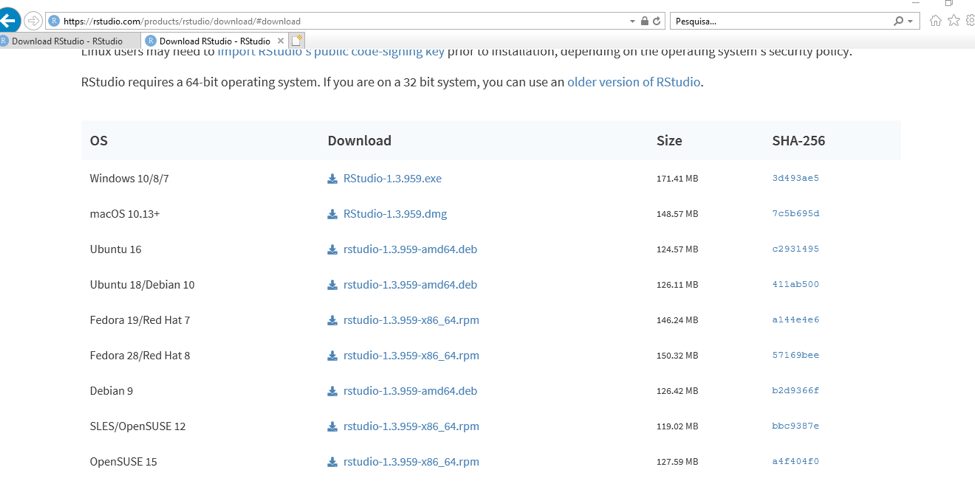
\includegraphics[width=13.54in]{img/inst_1_rstudio}

\begin{itemize}
\tightlist
\item
  Passo 3: Encontre o sistema operacional do seu computador (Ubuntu, Fedora, Debian ou OpenSUSE) e faça download.\\
\item
  Passo 4: Acesse o terminal na pasta onde foi feito o download e siga as instruções abaixo usando Fedora ou Ubuntu:

  \begin{itemize}
  \tightlist
  \item
    Fedora: \texttt{r\ sudo\ dnf\ install\ nomedo\_arquivo\_baixado.rpm}; Ex: \texttt{r\ sudo\ dnf\ install\ rstudio-1.3.959-x86\_64.rpm}
  \item
    Ubuntu: \texttt{r\ sudo\ dpkg\ -i\ nomedo\_arquivo\_baixado.deb}\\
  \end{itemize}
\item
  Passo 5: Após isso, o RStudio estará instalado no seu computador e pronto para uso.
\end{itemize}

\hypertarget{mac-os-x}{%
\section{Mac OS X}\label{mac-os-x}}

\hypertarget{instalar-o-r-1}{%
\subsection{Instalar o R}\label{instalar-o-r-1}}

\begin{itemize}
\tightlist
\item
  Passo 1: Abra o site \href{https://cran.r-project.org/}{CRAN - https://cran.r-project.org/}
\item
  Passo 2: Clique em Download de R for (Mac) OS X.\\
\item
  Passo 3: Clique duas vezes no arquivo depois de baixado que será instalado no seu computador.
\end{itemize}

\hypertarget{instalar-o-rstudio-1}{%
\subsection{Instalar o RStudio}\label{instalar-o-rstudio-1}}

\begin{itemize}
\tightlist
\item
  Passo 1: Acesse o site \url{https://rstudio.com/products/rstudio/download/}\\
\item
  Passo 2: Encontre na página o local de download gratuito conforme figura abaixo:
\end{itemize}

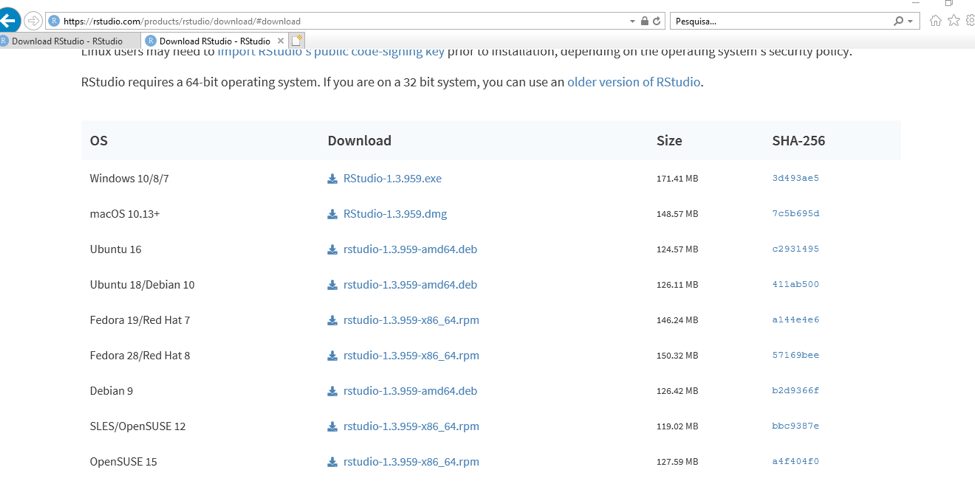
\includegraphics[width=13.54in]{img/inst_1_rstudio}

\begin{itemize}
\tightlist
\item
  Passo 3: Encontre o sistema operacional do seu computador (Mac OS) e faça download.\\
\item
  Passo 4: Depois de baixado, clique duas vezes no arquivo para instalá-lo. Após, estará pronto para uso.
\end{itemize}

\hypertarget{windows}{%
\section{Windows}\label{windows}}

\hypertarget{instalar-o-r-2}{%
\subsection{Instalar o R}\label{instalar-o-r-2}}

\begin{itemize}
\tightlist
\item
  Passo 1: Clique no seguinte link \url{https://cran.r-project.org/bin/windows/base/}\\
\item
  Passo 2: Clique em Download R for Windows (os números que aparecem nesse arquivo de download correspondem à versão do R disponível):
\end{itemize}

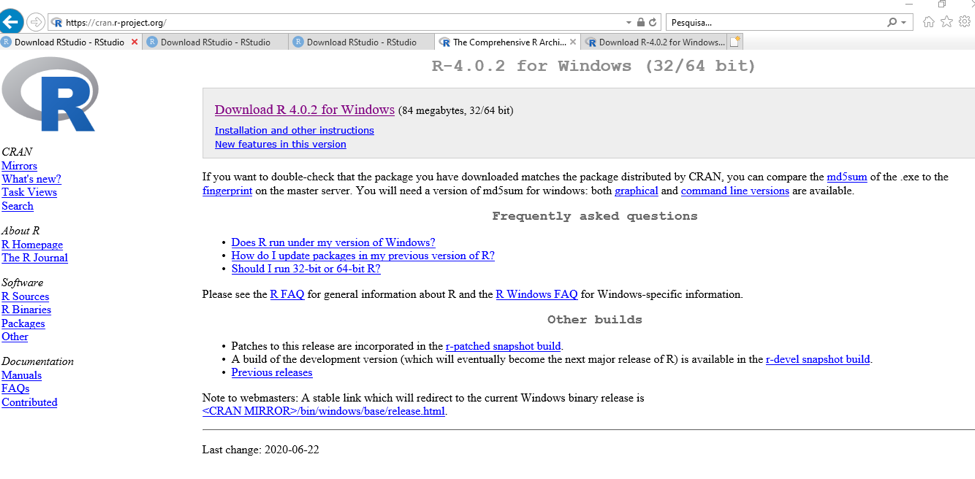
\includegraphics[width=13.54in]{img/inst_1_rwindows}

\begin{itemize}
\tightlist
\item
  Passo 3: Clique duas vezes no arquivo depois de baixado, clique em avançar até finalizar a instalação que será instalado no seu computador.
\end{itemize}

\hypertarget{instalar-o-rstudio-2}{%
\subsection{Instalar o RStudio}\label{instalar-o-rstudio-2}}

\begin{itemize}
\tightlist
\item
  Passo 1: Acesse o site \url{https://rstudio.com/products/rstudio/download/}\\
\item
  Passo 2: Encontre na página o local de download gratuito conforme figura abaixo:
\end{itemize}

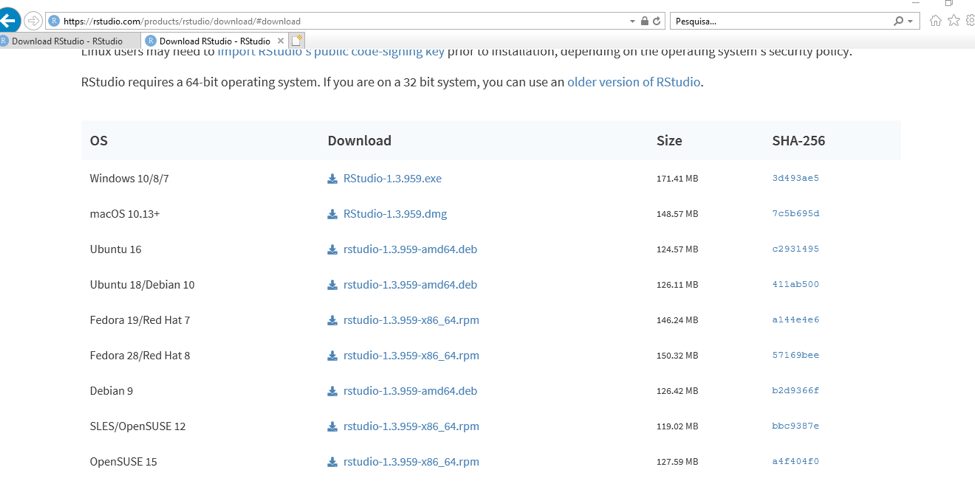
\includegraphics[width=13.54in]{img/inst_1_rstudio}

\begin{itemize}
\tightlist
\item
  Passo 3: Encontre o sistema operacional do seu computador (Windows) e faça download.
\item
  Passo 4: Depois de baixado, clique duas vezes no arquivo para instalá-lo. Após, estará pronto para uso.
\end{itemize}

\hypertarget{carregar-bibliotecas}{%
\chapter{Carregar Bibliotecas}\label{carregar-bibliotecas}}

Para carregar as bibliotecas

\begin{Shaded}
\begin{Highlighting}[]
\CommentTok{# carregar o tidyverse}
\KeywordTok{library}\NormalTok{(}\StringTok{"tidyverse"}\NormalTok{)}

\CommentTok{# carregar o codebook}
\KeywordTok{library}\NormalTok{(}\StringTok{"codebook"}\NormalTok{)}
\end{Highlighting}
\end{Shaded}

\hypertarget{gerar-dicionuxe1rio-de-variuxe1veis}{%
\section{Gerar dicionário de variáveis}\label{gerar-dicionuxe1rio-de-variuxe1veis}}

\begin{Shaded}
\begin{Highlighting}[]
\CommentTok{# gerar o dicionário de variáveis usando codebook}
\KeywordTok{label_browser_static}\NormalTok{(df_wvs7)}
\NormalTok{dicionario <-}\StringTok{ }\KeywordTok{codebook_table}\NormalTok{(wvs_bra)}
\end{Highlighting}
\end{Shaded}

\hypertarget{importar-a-base-de-dados}{%
\chapter{Importar a base de dados}\label{importar-a-base-de-dados}}

Acessar o \href{http://www.worldvaluessurvey.org/WVSContents.jsp}{Site do WVS}, baixar a versão desejada\ldots{} etc.

\begin{Shaded}
\begin{Highlighting}[]
\KeywordTok{load}\NormalTok{(}\StringTok{"./material/data/WVS_7.RData"}\NormalTok{)}\CommentTok{#abrir dados no formato R}

\NormalTok{wvs_bra <-}\StringTok{ }\KeywordTok{read_sav}\NormalTok{(}\StringTok{"material/data/WVS7_BRA_v2012.sav"}\NormalTok{)}\CommentTok{#importar dados formato SPSS}
\end{Highlighting}
\end{Shaded}

\hypertarget{descrever-e-analisar-os-dados}{%
\chapter{Descrever e Analisar os dados}\label{descrever-e-analisar-os-dados}}

\hypertarget{descrever-os-dados}{%
\section{Descrever os dados}\label{descrever-os-dados}}

Criar variáveis, vetores

Funções:
Filter: filtrar observações baseadas em uma condição
Select: escolher variáveis
Count: conta e cruza variáveis
Mutate: criar nova coluna
Summarise: resumir dados baseados em uma operação
Excluir missing values
Group: agrupar variáveis
View: visualizar variáveis escolhidas

Fazer gráficos
Criar anotacoes

\begin{Shaded}
\begin{Highlighting}[]
\OperatorTok\StringTok{ }\CommentTok{#conecta linhas do seu codigo}

\KeywordTok{filter}\NormalTok{() }\CommentTok{#filtrar observacoes baseado em uma condicao Brasil: filter(S003 == 76)}
\KeywordTok{select}\NormalTok{() }\CommentTok{#selecionar somente pais e sexo select(X001)}
\KeywordTok{count}\NormalTok{() }\CommentTok{# conta e cruza variaveis}
\KeywordTok{mutate}\NormalTok{() }\CommentTok{#cria uma nova coluna mutate(c = a + b)}
\KeywordTok{summarise}\NormalTok{() }\CommentTok{#resumir os nossos dados baseados em uma operacao summarise(media = mean(IDADE))}
\CommentTok{#na.rm mean() sd() median()}

\CommentTok{# exemplos }
\NormalTok{df_wvs7 }\OperatorTok\StringTok{ }\KeywordTok{summarise}\NormalTok{(}\DataTypeTok{media =} \KeywordTok{mean}\NormalTok{(X003, }\DataTypeTok{na.rm =} \OtherTok{TRUE}\NormalTok{))}

\CommentTok{# exemplos}
\NormalTok{df_wvs7 }\OperatorTok\StringTok{ }\KeywordTok{count}\NormalTok{(S003, X001)}
\end{Highlighting}
\end{Shaded}

\hypertarget{analises-bi-e-multi-variadas}{%
\section{Analises bi e multi-variadas}\label{analises-bi-e-multi-variadas}}

Cor: correlacionar
Regressao linear multipla: lm(variaveis)

\begin{Shaded}
\begin{Highlighting}[]
\CommentTok{#correlacao}
\NormalTok{df_wvs7 }\OperatorTok\StringTok{ }\KeywordTok{select}\NormalTok{(X002, X003) }\OperatorTok\StringTok{ }\KeywordTok{cor}\NormalTok{(}\DataTypeTok{use =} \StringTok{"complete.obs"}\NormalTok{)}

\CommentTok{#regressao linear multipla}

\NormalTok{resultado <-}\StringTok{ }\NormalTok{df_wvs7 }\OperatorTok\StringTok{ }\KeywordTok{group_by}\NormalTok{(S003) }\OperatorTok\StringTok{ }\KeywordTok{lm}\NormalTok{(X047 }\OperatorTok{~}\StringTok{ }\KeywordTok{scale}\NormalTok{(X025R) }\OperatorTok{+}\StringTok{ }\KeywordTok{scale}\NormalTok{(X002), }\DataTypeTok{data =}\NormalTok{ .)}
\NormalTok{resultado_bol <-}\StringTok{ }\NormalTok{df_wvs7 }\OperatorTok\StringTok{ }\KeywordTok{filter}\NormalTok{(S003 }\OperatorTok{==}\StringTok{ }\DecValTok{68}\NormalTok{) }\OperatorTok\StringTok{ }\KeywordTok{lm}\NormalTok{(X047 }\OperatorTok{~}\StringTok{ }\KeywordTok{scale}\NormalTok{(X025R) }\OperatorTok{+}\StringTok{ }\KeywordTok{scale}\NormalTok{(X002), }\DataTypeTok{data =}\NormalTok{ .)}

\NormalTok{bra <-}\StringTok{ }\KeywordTok{summary}\NormalTok{(resultado)}\OperatorTok{$}\NormalTok{coeff}
\NormalTok{bol <-}\KeywordTok{summary}\NormalTok{(resultado_bol)}\OperatorTok{$}\NormalTok{coeff}

\KeywordTok{glm}\NormalTok{(binaria }\OperatorTok{~}\StringTok{ }\NormalTok{expicacao1 }\OperatorTok{+}\StringTok{ }\NormalTok{explicacao2, }\DataTypeTok{data =}\NormalTok{ wvs7)}
\end{Highlighting}
\end{Shaded}

\hypertarget{visualizar-os-dados}{%
\chapter{Visualizar os dados}\label{visualizar-os-dados}}

ggplot2

\hypertarget{glossuxe1rio}{%
\chapter{Glossário}\label{glossuxe1rio}}

\begin{itemize}
\tightlist
\item
  Estatística:

  \begin{itemize}
  \tightlist
  \item
    variáveis numéricas
  \item
    categóricas
  \end{itemize}
\item
  Programação:

  \begin{itemize}
  \tightlist
  \item
    variável
  \item
    objeto
  \item
    vetor
  \item
    lista
  \item
    dataframe
  \item
    script
  \item
    console
  \item
    environment
  \item
    arquivos
  \item
    Códigos-chave
  \end{itemize}
\item
  Verbos:

  \begin{itemize}
  \tightlist
  \item
    count
  \item
    select
  \item
    filter
  \item
    view
  \item
    summarise
  \item
    mutate
  \end{itemize}
\end{itemize}

  \bibliography{tutorial.bib,packages.bib}

\end{document}
